\newpage
\appendix
\section{FEA model: Vertical displacements of boundary conditions}
\begin{table}[!hbt]
\centering
\begin{tabular}{|l|l|}
\hline
\textbf{Width of mesh} & \textbf{Displacement(mm)} \\ \hline
1 & 0.03 \\ \hline
2 & 0.13 \\ \hline
3 & 0.29 \\ \hline
4 & 0.51 \\ \hline
5 & 0.80 \\ \hline
6 & 1.14 \\ \hline
7 & 1.55 \\ \hline
8 & 2.01 \\ \hline
9 & 2.53 \\ \hline
10 & 3.10 \\ \hline
11 & 3.72 \\ \hline
12 & 4.39 \\ \hline
13 & 5.11 \\ \hline
14 & 5.87 \\ \hline
15 & 6.67 \\ \hline
16 & 7.50 \\ \hline
17 & 8.37 \\ \hline
18 & 9.26 \\ \hline
19 & 10.18 \\ \hline
20 & 11.12 \\ \hline
21 & 12.07 \\ \hline
22 & 13.04 \\ \hline
23 & 14.02 \\ \hline
24 & 15.00 \\ \hline
\end{tabular}
\caption{Displacements used to flatten the root}
\label{tab:disp}
\end{table}

\begin{figure}[!hbt]
     \centering
     \begin{subfigure}[b]{0.4\textwidth}
         \centering
         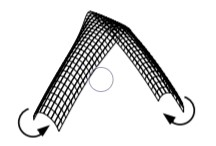
\includegraphics[width=\textwidth]{images/samesense.JPG}
         \caption{Same-sense bending of tapespring}
         \label{fig:same}
     \end{subfigure}
     \hfill
     \begin{subfigure}[b]{0.4\textwidth}
         \centering
         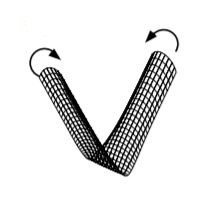
\includegraphics[width=\textwidth]{images/oppsense.JPG}
         \caption{Opposite-sense bending of tapespring}
         \label{fig:opp}
     \end{subfigure}
     \caption{Bending conventions}
     \end{figure}

\newpage
\section{Fitted curves error for ploy lengths}
\begin{table}[!hbt]
\centering
\begin{tabular}{|ll|l|l|l|l|}
\cline{3-6}
\multicolumn{1}{c}{} & \multicolumn{1}{c|}{} & \multicolumn{2}{c|}{\textbf{First order}} & \multicolumn{2}{c|}{\textbf{Second order}} \\ \hline
\multicolumn{1}{|c|}{\textbf{\begin{tabular}[c]{@{}c@{}}Clamp width \\ (mm)\end{tabular}}} &
\multicolumn{1}{c|}{\textbf{\begin{tabular}[c]{@{}c@{}}Ploy length \\ (mm)\end{tabular}}} & \multicolumn{1}{c|}{\textbf{\begin{tabular}[c]{@{}c@{}}Curve fit \\ values\end{tabular}}} & \multicolumn{1}{c|}{\textbf{\begin{tabular}[c]{@{}c@{}}Fit error \\ percentage\end{tabular}}} & \multicolumn{1}{c|}{\textbf{\begin{tabular}[c]{@{}c@{}}Curve fit\\  values\end{tabular}}} & \multicolumn{1}{c|}{\textbf{\begin{tabular}[c]{@{}c@{}}Fit error \\ percentage\end{tabular}}} \\ \hline
\multicolumn{1}{|l|}{45.16} & 197.00 & 216.49 & 9.89 & 191.67 & -2.71 \\ \hline
\multicolumn{1}{|l|}{43.20} & 197.00 & 211.60 & 7.41 & 193.26 & -1.90 \\ \hline
\multicolumn{1}{|l|}{41.23} & 196.00 & 206.71 & 5.47 & 194.26 & -0.89 \\ \hline
\multicolumn{1}{|l|}{39.27} & 195.00 & 201.83 & 3.50 & 194.67 & -0.17 \\ \hline
\multicolumn{1}{|l|}{37.31} & 193.00 & 196.94 & 2.04 & 194.49 & 0.77 \\ \hline
\multicolumn{1}{|l|}{35.34} & 191.00 & 192.05 & 0.55 & 193.72 & 1.42 \\ \hline
\multicolumn{1}{|l|}{33.38} & 190.00 & 187.17 & -1.49 & 192.37 & 1.25 \\ \hline
\multicolumn{1}{|l|}{31.42} & 187.00 & 182.28 & -2.52 & 190.42 & 1.83 \\ \hline
\multicolumn{1}{|l|}{29.45} & 184.00 & 177.39 & -3.59 & 187.89 & 2.11 \\ \hline
\multicolumn{1}{|l|}{27.49} & 179.00 & 172.51 & -3.63 & 184.77 & 3.22 \\ \hline
\multicolumn{1}{|l|}{25.53} & 180.00 & 167.62 & -6.88 & 181.06 & 0.59 \\ \hline
\multicolumn{1}{|l|}{23.56} & 171.00 & 162.73 & -4.83 & 176.76 & 3.37 \\ \hline
\multicolumn{1}{|l|}{21.60} & 172.00 & 157.85 & -8.23 & 171.88 & -0.07 \\ \hline
\multicolumn{1}{|l|}{19.63} & 163.00 & 152.96 & -6.16 & 166.40 & 2.09 \\ \hline
\multicolumn{1}{|l|}{17.67} & 162.00 & 148.08 & -8.60 & 160.34 & -1.03 \\ \hline
\multicolumn{1}{|l|}{15.71} & 154.00 & 143.19 & -7.02 & 153.69 & -0.20 \\ \hline
\multicolumn{1}{|l|}{13.74} & 149.00 & 138.30 & -7.18 & 146.44 & -1.72 \\ \hline
\multicolumn{1}{|l|}{11.78} & 145.00 & 133.42 & -7.99 & 138.61 & -4.40 \\ \hline
\multicolumn{1}{|l|}{9.82} & 128.00 & 128.53 & 0.41 & 130.20 & 1.72 \\ \hline
\multicolumn{1}{|l|}{7.85} & 128.00 & 123.64 & -3.40 & 121.19 & -5.32 \\ \hline
\multicolumn{1}{|l|}{5.89} & 131.00 & 118.76 & -9.35 & 111.60 & -14.81 \\ \hline
\multicolumn{1}{|l|}{3.93} & 109.00 & 113.87 & 4.47 & 101.41 & -6.96 \\ \hline
\multicolumn{1}{|l|}{1.96} & 106.00 & 108.98 & 2.81 & 90.64 & -14.49 \\ \hline
\end{tabular}
\caption{Error percentage of first order and second order curves}
\end{table}
\section{Maximum reaction moment for changing width of clamp}
\begin{table}[!hbt]
\centering
\begin{tabular}{|c|c|}
\hline
\multicolumn{1}{|c|}{\textbf{\begin{tabular}[c]{@{}c@{}}Width of \\ the clamp (mm)\end{tabular}}} & \multicolumn{1}{c|}{\textbf{\begin{tabular}[c]{@{}c@{}}Maximum reaction \\ moment\ (Nmm)\end{tabular}}} \\ \hline
48 & 31.5 \\ \hline
38 & 47.7 \\ \hline
32 & 78.5 \\ \hline
14 & 105 \\ \hline
8 & 157 \\ \hline
\end{tabular}
\caption{\label{tab:rotwidth}Maximum reaction moment and width of the clamp}
\end{table}

\newpage
\section{Calladine shell theory}
\begin{figure}[!hbt]
    \centering
    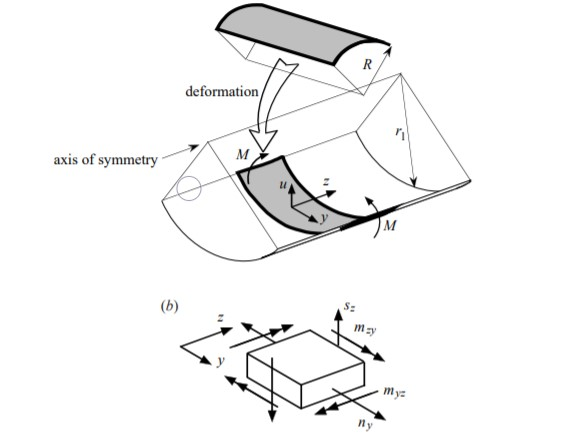
\includegraphics{images/mansfieldtheory.jpg}
    \caption{Calladine shell theory from source \cite{Seffen1999}}
    \label{fig:mansfield}
\end{figure}

\begin{figure}[!hbt]
    \centering
    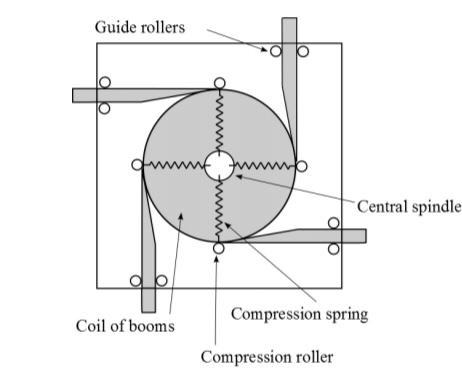
\includegraphics[height=6cm]{images/guiderollers.jpg}
    \caption{Position of guiderollers in STEM boom deployers from source \cite{Hoskin2015}}
    \label{fig:guiderollers}
\end{figure}


